\chapter{Opis projektnog zadatka}

\iffalse % block comment (zavrsava sa fi)

        \textit{Na osnovi projektnog zadatka detaljno opisati korisničke zahtjeve. Što jasnije opisati cilj projektnog zadatka, razraditi problematiku zadatka, dodati nove aspekte problema i potencijalnih rješenja. Očekuje se minimalno 3, a poželjno 4-5 stranica opisa.	Teme koje treba dodatno razraditi u ovom poglavlju su:}
		\begin{packed_item}
			\item \textit{potencijalna korist ovog projekta}
			\item \textit{postojeća slična rješenja (istražiti i ukratko opisati razlike u odnosu na zadani zadatak). Dodajte slike koja predočavaju slična rješenja.}
			\item \textit{skup korisnika koji bi mogao biti zainteresiran za ostvareno rješenje.}
			\item \textit{mogućnost prilagodbe rješenja }
			\item \textit{opseg projektnog zadatka}
			\item \textit{moguće nadogradnje projektnog zadatka}
		\end{packed_item}
		
		\textit{Za pomoć pogledati reference navedene u poglavlju „Popis literature“, a po potrebi konzultirati sadržaj na internetu koji nudi dobre smjernice u tom pogledu.}\vspace{0.5cm}
		
\fi % block comment (pocinje sa iffalse)
		
		\section{Opis problematike}
		
		{Porastom broja neprofitnih organizacija iz godine u godinu, raste i potreba za kvalitetnim aplikacijama koje bi takvim organizacijama omogućile nesmetan rad i funkcioniranje. Kako takve organizacije nisu u mogućnosti samostalno postići zadovoljavajuću razinu prihoda, to im postaje najveći problem te primorane su na suradnju s kompanijama sponzorima.}\vspace{0.3cm}

		{Odaziv sponzora je često vrlo malen te je stoga potrebno kontaktirati velik broj kompanija. Praćenje statusa suradnji (uspješne / neuspješne) i osoba zaduženih za kontaktiranje sponzora vrlo brzo postaje kompleksno i neefikasno, a također dolazi i do mogućnosti curenja informacija. Raste potreba za aplikacijom koja će omogućiti evidenciju navedenih stavki te korisnicima dodijeliti razinu ovlasti kako bi umanjili mogućnost curenja informacija.}
		
		\section{Postojeća rješenja}
		
		{Najraširenije rješenje koje danas koriste gotovi svi jesu tablice. Bilo to u MS Excelu za jednokorisnički ili Google sheets \ref{fig:GoogleSheets} za višekorisnički rad, tablice su jedan od najboljih načina prikaza velikog broja podataka. Nažalost, ova rješenja imaju gore navedene probleme te stoga nisu pogodna za upotrebu na razini veće organizacije.}
		
		\begin{figure}[H]
			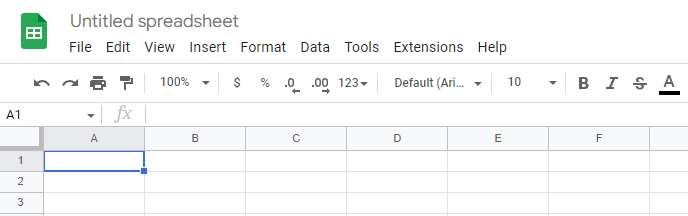
\includegraphics[width=\textwidth]{slike/GoogleSheets.png} %veličina u odnosu na širinu linije
			\caption{Prikaz alata Google sheets}
			\label{fig:GoogleSheets} %label mora biti drugaciji za svaku sliku
		\end{figure}
		
		\section{Opseg projektnog zadatka}

		{Cilj ovog projekta je razviti programsku podršku za stvaranje web aplikacije \textit{”Company Database“} koja će služiti za evidenciju statusa suradnje kompanija na projektima i jednostavan uvid od strane \underbar{ovlaštenih} korisnika.}\vspace{0.2cm}
		
		{Korisnici će se u web aplikaciju prijavljivati koristeći Google račun koji mora biti registriran od strane drugih korisnika putem web aplikacije. Svaki je korisnik definiran sljedećim parametrima:}
		\begin{packed_item}
			\item {ime}
			\item {prezime}
			\item {korisničko ime} (nadimak)
			\item {opis}
			\item {email za login u aplikaciju}
			\item {email za obavijesti}
			\item {najviša razina ovlasti koju posjeduje (ako ima više razina ovlasti)}
		\end{packed_item}
		
		{Razlikovat ćemo 5 razina ovlasti, a to su redom od najviše prema najnižoj:}
		\begin{packed_item}
			\item {Administrator}
			\item {Moderator}
			\item {Fundraising (FR) responsible}
			\item {Fundraising (FR) team member}
			\item {Observer}
		\end{packed_item}

		{Svaki korisnik određene razine ovlasti ima sve mogućnosti svoje i svih nižih razina ovlasti sustava. Također ima mogućnost (kroz određene akcije) dodjeljivanja i oduzimanja \underbar{razina ovlasti} korisnicima nižih razina od svoje.}

		{Iznimke su administrator koji može dodijeliti i oduzeti i ostalim administratorima sustava te FR team member koji ne može dodijeliti niti oduzeti ovlasti jer se observer automatski dodjeljuje svim korisnicima koja nemaju višu razinu ovlasti.}\vspace{0.3cm}
		
		{\underbar{Projekt} je obilježen nazivom, kategorijom, tipom (interni ili eksterni), datumom početka i kraja, FR responsible-om zaduženim za navedeni projekt, popisom FR team member-a, FR ciljem (željeni prihod od projekta), prvim i drugom „pingom“ (timestamp) te popisom kompanija s kojima se surađuje na tom projektu.}\vspace{0.1cm}

		{\underbar{Kompanija} je obilježena nazivom, područjem kojim se bavi (npr. IT), ABC kategorizacijom, mjesecom planiranja budžeta, državom, poštanskim brojem, gradom, adresom, linkom na web stranicu, kratkim opisom, boolean varijablom \textit{„kontaktirati“} (koja označava treba li tu tvrtku u budućnosti kontaktirati) te popisom zaposlenika.}\vspace{0.1cm}
		
		{\underbar{Popis kompanija} moguće je uzlazno i silazno sortirati prema nazivu, području, mjesecu planiranja budžeta i linku na web stranicu te pretraživati po nazivu.}\vspace{0.1cm}

		{\underbar{Zaposlenik} kao entitet pripada kompaniji, a definiran je imenom, prezimenom, email adresom, brojem mobitela, ulogom u kompaniji (npr. CEO) te kratkim opisom.}\vspace{0.1cm}

		{\underbar{Suradnja} predstavlja poveznicu između projekta i kompanije, a obilježena je odgovornom osobom (koja je za nju zadužena), kontaktiranom osobom u kompaniji, kategorijom (financijska, materijalna ili akademska suradnja), vlastitim statusom (kontaktirano, ping, dopis, sastanak, uspješno ili neuspješno), komentarom (tj. sažetkom suradnje) te vrijednošću suradnje (koje se sumiraju i popunjavaju FR cilj projekta).}\vspace{0.3cm}

		{Aplikacija, sa svim navedenim funkcionalnostima i specifičnostima, bit će izvedena kao web aplikacija kojoj korisnici pristupaju pomoću Google autentifikatora. Bit će jednostavna za korištenje zahvaljujući preglednom i intuitivnom sučelju. Sustav će podržavati rad više korisnika u stvarnom vremenu, frontend će biti ostvaren u React-u, a backend će koristiti relacijsku bazu podataka i Spring boot.}
		
		
		\section{Mogućnost prilagodbe rješenja}
		
		{Kako bi što više ljudi moglo znati za projekt, organizatori nerijetko kontaktiraju razne medije kako zainteresirani ne bi propustili priliku. Slična aplikacija bi se također mogla koristiti za komunikaciju s medijima. Entitet Tvrtka bi bilo bi potrebno izmijeniti u Medij zajedno s odgovarajućim atributima, dok bi u entitetu Suradnja bilo potrebno izmijeniti samo atribute.}\vspace{0.1cm}
		
		{Ovakva bi aplikacija bila od koristi ne samo neprofitnim organizacijama, već i svima koji organiziraju nešto što treba publicitet.}
		
		\section{Mogućnost nadogradnje rješenja}
		
		{Aplikacija bi se dodatno mogla nadograditi proširenjem komentara suradnje, primarno u svrhu prenošenja znanja od iskusniji osoba. Te bi osobe kroz komentar na suradnju mogli dati svoj input vezano uz neku temu. Tada bi i korisnik koji je odgovoran za suradnju dobio te obavijesti na naslovnicu.}\vspace{0.1cm}
		
		{Nadalje, aplikacija bi mogla, osim tabličnog, podržavati više načina prikaza podataka o korisnicima, projektima, tvrtkama i suradnjama. Možda bi ih se moglo grupirati temeljem nekih postojećih ili novih atributa te onda to iskoristiti.}\vspace{0.1cm}
		
		{Također bi bilo korisno uvesti dodatne mogućnosti filtriranja svih tablica i drugih načina prikaza podataka.}\vspace{0.1cm}
		
		{Ako se projekti neke organizacije ponavljaju iz godine u godinu, bilo bi korisno uvesti neki način kopiranja podataka iz tablice prošlogodišnjeg projekta. Korisno bi bilo dodati i mogućnost izvoza i uvoz podataka iz i u tablice u JSON i CSV formatima.}\vspace{0.1cm}
		
		{Kako bi se još više smanjila mogućnost curenja informacija, mogao bi se uvesti tzv. soft lock korisnika koji bi očuvao podatke o korisniku, ali mu onemogućio da se ulogira (npr. ako korisnik više nije dio organizacije).}\vspace{0.1cm}
		
		{Aplikaciju bi također bilo moguće spojiti s nekakvim internim sustavom za upravljanjem članovima organizacije.}\vspace{0.1cm}
		
		{Što se tiče UX-a, tu uvijek ima mjesta za napredak. Dodavanje animacija tokom prijelaza od jedne stranice na drugu ili važnije tokom dohvata podataka iz baze kako bi korisnik znao da se njegov zahtjev procesuira. Moglo bi se uvesti neki način prikaza uspješnosti odrade nekog zadatka (npr. dodavanje podatka u bazu).}
		
		{Mogao poboljšati i sam UI da aplikacija izgleda profesionalnije i bude ugodnija za korištenje, ali i kako bi aplikaciju mogle koristiti osobe s posebnim potrebama.}\vspace{0.1cm}

		\eject

\iffalse % block comment (zavrsava sa fi)

		\section{Primjeri u \LaTeX u}
		
		\textit{Ovo potpoglavlje izbrisati.}\\

		U nastavku se nalaze različiti primjeri kako koristiti osnovne funkcionalnosti \LaTeX a koje su potrebne za izradu dokumentacije. Za dodatnu pomoć obratiti se asistentu na projektu ili potražiti upute na sljedećim web sjedištima:
		\begin{itemize}
			\item Upute za izradu diplomskog rada u \LaTeX u - \url{https://www.fer.unizg.hr/_download/repository/LaTeX-upute.pdf}
			\item \LaTeX\ projekt - \url{https://www.latex-project.org/help/}
			\item StackExchange za Tex - \url{https://tex.stackexchange.com/}\\
		
		\end{itemize} 	

		%unos slike
		\begin{figure}[H]
			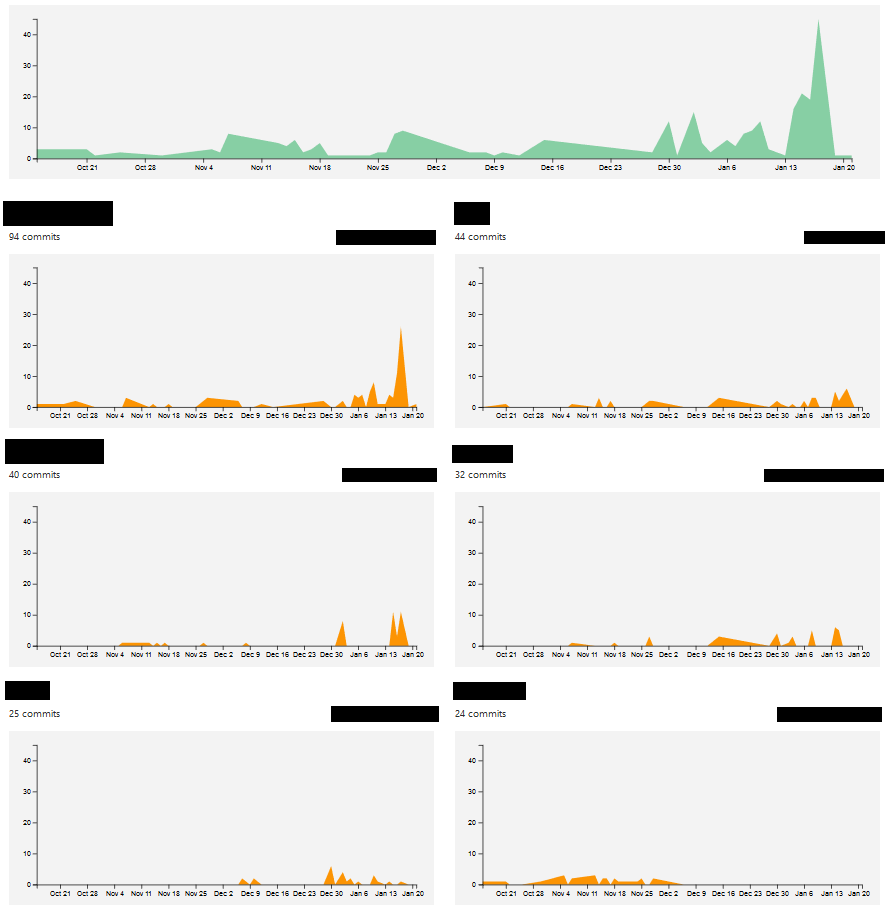
\includegraphics[scale=0.4]{slike/aktivnost.PNG} %veličina slike u odnosu na originalnu datoteku i pozicija slike
			\centering
			\caption{Primjer slike s potpisom}
			\label{fig:promjene}
		\end{figure}
		
		\begin{figure}[H]
			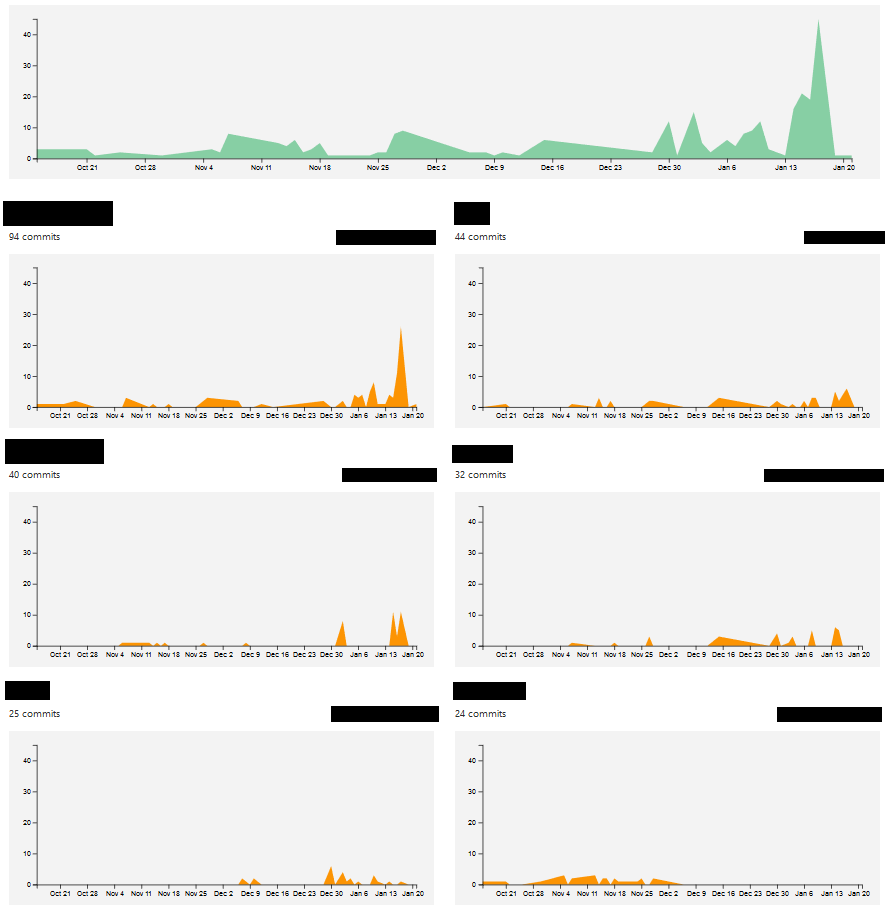
\includegraphics[width=\textwidth]{slike/aktivnost.PNG} %veličina u odnosu na širinu linije
			\caption{Primjer slike s potpisom 2}
			\label{fig:promjene2} %label mora biti drugaciji za svaku sliku
		\end{figure}
		
		Referenciranje slike \ref{fig:promjene2} u tekstu.
		\eject
		
\fi % block comment (pocinje sa iffalse)